% -----------------------------------------------
% Vlastní text práce (kapitoly práce)
% -----------------------------------------------

% -----------------------------------------------
\chapter{Mössbauer effect and spectroscopy}
% -----------------------------------------------
The Mössbauer effect is an interaction that can occur on atomic nuclei under certain circumstances. It is a recoilless resonance emission/absorption of gamma photons by nuclei of the source/absorber with discrete nuclear energy levels. This effect has a special application in material science - Mössbauer spectroscopy (MS), which is a nuclear experimental technique and a special type of gamma spectroscopy that uses the appropriate nuclei in the sample as probes of local electric and magnetic fields. 

\par
This technique is capable of providing much unique information in material science, geology, chemistry and biology - study of phase and chemical composition of solid materials, study of local magnetic fields and spin states and in-situ measurements of phase transitions \cite{moss}. The main disadvantage of this technique is that there is no suitable radiation source for many isotopes. The most important is iron and its isotope $^{57}$Fe with the radioactive source $^{57}$Co (which decays to an excited state of $^{57}$Fe with a half-life of 271.81 days \cite{co57}), which allows Mössbauer spectroscopy to be used in many areas studying iron compounds.
%Mössbauer effect is an interaction, which can, under certain circumstances, occur on atomic nuclei. It is recoilless resonance emission/absorption of gamma photons by nuclei of source/absorber with discrete nuclear energy levels. This effect has a special application in the field of material research - the Mössbauer spectroscopy (MS), which is a nuclear experimental technique and a special type of gamma spectroscopy, which uses the appropriate nuclei in studied sample as probes of local electric and magnetic fields. 
%
%\par
%This technique is capable of providing many unique information in material research, geology, chemistry and biology - study of phase and chemical composition of solid materials, study of local magnetic fields and spin states and in-situ measurements of phase transitions \cite{moss}. The main disadvantage of this technique is the fact that there is not an appropriate radiation source for many isotopes. The major significance has iron and its isotope $^{57}$Fe with radioactive source $^{57}$Co (which decays into an excited state of $^{57}$Fe with half-life 271.81 days \cite{co57}), which allows the Mössbauer spectroscopy to be employed in many fields investigating iron compounds.

% -----------------------------------------------
\section{Physical concept}

\subsection{Resonace emission and absorption}
In the previous chapters it was mentioned that atomic nuclei are quantum systems with discrete energy levels (analogous to the energy levels of the electron shell), so upon de-excitation or excitation they emit/absorb gamma photons with energy $E_0$ equal to the difference between the levels. The emitted/absorbed energy spectra follow the shape of the Lorentzian curve. 
\par
However, these emitted/absorbed energy spectra are altered due to the momentum conservation law. Part of the gamma photon energy is transferred to the kinetic energy of the nucleus, the crystal as a whole body, or transformed into lattice vibrations (phonons). 
In the case of a free, stationary nucleus, the momentum and energy transfers are so large that the emission and absorption spectra are shifted in different directions by large energetic values, making resonance absorption impossible to observe. However, the case of the nucleus bounded in the crystal lattice is different - the crystal as a whole body will absorb the momentum. If we consider that the whole crystal has a much larger mass than the nucleus, the energy transfer into the kinetic energy of the crystal will be negligible - the gamma photon energy remains unchanged and this results in recoilless emission/absorption. In this case the emission and absorption energy spectra overlap and this makes resonance absorption (Mössbauer effect) observable \cite{moss}.
%In previous chapters was mentioned, that the atomic nuclei are quantum systems with discrete energy levels (analogous to the energy levels of electron shell), thus upon deexcitation or excitation they emit/absorb gamma photon with energy $E_0$ equal to the difference between the levels. The emitted/absorbed energy spectra follow the shape of Lorentzian curve. 
%\par
%However, these emitted/absorbed energy spectra are altered due to the  momentum conservation law. Part of the gamma photon energy is transferred to the  kinetic energy of nucleus, crystal as whole body or is transformed into lattice vibrations (phonons). 
%In the case of free, stationary nucleus, momentum and energy transfers are so high, that the emission and absorption spectra are shifted to different directions by large energetic values, which makes the resonance absorption impossible to observe. However, the nucleus bounded into the crystal lattice is a different case - the crystal as whole body will absorb the momentum. If we consider, that the entire crystal has much larger mass than the nucleus, the energy transfer into kinetic energy of the crystal will be negligible - the gamma photon energy remains unaltered and that results into recoilless emission/absorption. In this case the  emission and absorption energy spectra have overlap and that makes the resonance absorption (Mössbauer effect) observable \cite{moss}.

\subsection{Interaction of nuclei with local fields}
The nucleus, bounded within the lattice and surrounded by electrons arranged according to the chemical bonds, has perturbed energy levels. These perturbed energy levels are a consequence of the interactions of the nucleus with local electric and magnetic fields, resulting in each phase or chemical composition having its own nuclear emission/absorption spectrum - the Mössbauer spectrum. Quantum physics has very well known calculation techniques to describe these variations in energy spectra - perturbation theory.

\par
The main properties of a nucleus that cause the interactions with local electric and magnetic fields are: the atomic number $Z$, the quadrupole moment $Q$ and its spin $I$ along with its projections. For spectroscopy there are three main hyperfine interactions \cite{moss}:

\begin{itemize}
\item Electric monopole interaction - the interaction between the protons of the nucleus and the s-electrons (which have a non-zero probability of being in the nucleus). It results in an isomeric shift of the energy levels $\delta = E_M - E_0$. The $\delta$ must be defined with respect to a fixed energy level, for example the level of the radioactive source that is used. This type of MS spectrum has a shape consisting of only one Lorentzian (singlet shape).
\item Electric quadrupole interaction - the inhomogeneous electric field inside the nucleus interacts with the quadrupole momentum $Q$ of the nuclei. It results in energy variations with respect to the square of the magnetic quantum number $E_Q \sim m^{2}$ - the states allowing different values of $|m|$ are split into sub-states. For $m = \pm 1/2$ there are two Lorentzians in the MS spectra - dublet.
\item Magnetic dipole interaction - the spin $I$ is tied to the magnetic momentum by the relation $\mu = \gamma I$, where $\gamma$ is a gyromagnetic ratio. This magnetic momentum interacts with magnetic fields in the nucleus and leads to the nuclear Zeeman effect - the splitting of states with respect to possible values of the magnetic quantum number $m$. The magnetic dipole interaction plays an important role in studying the magnetic properties of materials.
\end{itemize}
Each of these effects can occur separately or simultaneously with the others.
%The nucleus bounded inside the lattice surrounded by electrons arranged according to the chemical bonds has perturbed energy levels. These perturbed energy levels are consequences of the interactions of nucleus with local electric and magnetic fields, resulting in each phase or chemical composition has its own nuclear emission/absorption spectrum - the Mössbauer spectrum. The quantum physics has very-well known computation techniques to describe these variations in energy spectra - the perturbation theory.
%
%\par
%The main properties of nucleus which induces the interactions with local electric and magnetic fields are: atomic number $Z$, quadrupole momentum $Q$ and its spin $I$ along with its projections. For spectroscopy there are three main hyperfine interactions \cite{moss}:
%
%\begin{itemize}
%\item Electric monopole interaction - the interaction between the protons of nucleus and the s-electrons (which have non-zero probability of being found inside nucleus). It results into isomer shift of energy levels $\delta = E_M - E_0$. The $\delta$ has to be defined with respect to some fixed energy level, for example to the level of the used radioactive source. This type of MS spectra has shape consisting of only one Lorentzian (singlet shape).
%\item Electric quadrupole interaction - the inhomogeneous electric field inside nucleus interacts with the quadrupole momentum $Q$ of the nuclei. It results into energy variations with respect to the square of magnetic quantum number $E_Q \sim m^{2}$- the states which allows different values of $|m|$ are splitted into sub-states. For $m = \pm 1/2$ there are two Lorentzians in MS spectra - dublet. 
%\item Magnetic dipole interaction - the spin $I$ is tied up with magnetic momentum via relation $\mu = \gamma I$, where $\gamma$ is a gyromagnetic ratio. This magnetic momentum interacts with magnetic fields inside nucleus and results into nuclear Zeeman effect - the splitting of the states with respect to possible values of magnetic quantum number $m$. The magnetic dipole interaction has a significant role when it comes to study the magnetic properties of materials.
%\end{itemize}
%Each of these effects can occur separately or simultaneously with the others.


% -----------------------------------------------



\section{Mössbauer spectroscopy}
To obtain the spectra, we can use one of several measurement setups with given geometries. In laboratories there are dominant the setups employing transmission or backscattering geometry with the sample as the absorber and with Doppler modulation of the gamma photon energy. The emitted photons or other products generated by the excitation are detected by a detector with electronics to accumulate the Mössbauer spectra. The source is attached to the Doppler modulation unit (transducer) and the energy of the gamma photons is modulated by the relative velocity of the source and absorber, typically in the range of about $\pm$ 1 $\mu$eV.
\par
For the transmission geometry, the key concept of the measurement is that if we irradiate the sample placed as an absorber with gamma photons with energy varied by the Doppler modulation, the gamma photons with energy equal to one of the transitions (resonance energies) will be absorbed with a certain probability. The detector is positioned behind the absorber and measures the number of gamma photons at a defined energy step. The minimum counts are measured around the resonance energy. The transmission geometry of Mössbauer spectra can be seen in the figure \ref{msspec}.
%To obtain the spectra, we can use one of the several measurement setups with given geometries. In laboratories there are dominant the setups employing transmission or backscattering geometry with sample as an absorber and with the Doppler modulation of the gamma photons energy. The transmitted photons or other products developed upon deexcitation are detected by appropriate detector with electronics to accumulate the Mössbauer spectra. The source is attached to the Doppler modulation unit (transducer), and by the relative velocity of source and absorber the energy of gamma photons is modulated typically in the range of about $\pm$ 1 $\mu$eV.
%\par
%For transmission geometry the key concept of measurement is that if we irradiate the sample placed as an absorber by gamma photons with energy varied by the Doppler modulation, the gamma photons with energy equal to one of the transitions (resonant energies) are absorbed with certain probability. The detector is situated behind the absorber and measures the number of gamma photons at defined energy step. The minimum counts are measured around the resonant energy. The transmission geometry Mössbauer spectra can be seen in the figure \ref{msspec}.
\par
The concept of a backscattering geometry is similar in many ways, but the main difference is the detection of the secondary particles. The nuclei in the sample are excited by appropriate gamma photons and subsequently decay back to the original state with some effects following - re-emission of the "original" gamma photons in a random direction, emission of electrons from the shell (ejected by deexcitation energy quanta, also called conversion electrons) followed by characteristic x-rays or possibly by auger electrons. The detection of electrons and X-rays instead of gamma photons has many advantages and disadvantages, and for certain applications the use of the backscattering geometry may be more appropriate. For example, the detection of conversion electrons could handle the surface characterisation of the sample due to the lower transmittance of electrons when compared to gamma photons.
%\par
%The concept of backscattering geometry is similar in many ways, but the main difference is the detection of the secondary particles. The nuclei in the sample are excited by appropriate gamma photons and subsequently, they decay back into the original state with some effects following - reemission of the "original" gamma photons in random direction, emission of electrons from the shell (ejected by deexcitation energy quanta, also called conversion electrons) followed by characteristic x-rays or possibly by auger electrons. The detection of electrons and x-rays instead of gamma photons have many advantages and disadvantages and for certain application, the usage of backscattering geometry could be more appropriate. For example, the detection of conversion electrons could handle the surface characterization of the sample due to the lower transmittance of electrons when compared to gamma photons.

\begin{figure}[H]
 \centering
 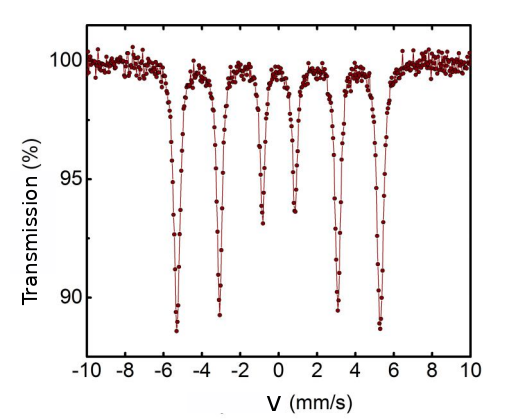
\includegraphics[scale=0.7, angle = 0]{./pictures/MSSpec.png}
 \caption{Transmission Mössbauer spectrum of $\alpha$-Fe. Taken and modified from \cite{NOVAK2016thesis}.}
 \label{msspec}
 
\end{figure}


\section{$^{57}$Fe spectroscopy}
One of the isotopes on which we are able to observe a Mössbauer effect is $^{57}$Fe (relative abundance only $2.119 \%$ \cite{compounds}). The source is $^{57}$Co, which decays into the second excited state of $^{57}$Fe by electron capture. The resulting $^{57}$Fe nuclei can deexcite themselves in two ways ( figure \ref{Fe57scheme}) - by direct deexcitation to the ground state by emission of 136.5 keV photon or by deexcitation to the first excited state by emission of 122.1 keV photon. The first excited state is essential as it is used to study the hyperfine interactions. After the lifetime of the first excited state, the 14.4 keV photon (or other possible conversion products) is emitted as it falls to the ground state. The $^{57}$Fe spectroscopy in transmission geometry is based on the detection of the 14.4 keV gamma photons. This thesis is mainly devoted to the application of semiconductor detectors for the detection of these 14.4 keV gamma photons. The $^{57}$Fe spectroscopy can also be performed in the backscattering geometry by detecting the conversion electrons or conversion X-rays with energies around 6.4 keV.
%One of the isotopes, on which we are capable to observe a Mössbauer effect is $^{57}$Fe (relative abundance only $2.119 \%$ \cite{compounds}). As a source is used $^{57}$Co, which decays into second excited state of $^{57}$Fe by electron capture. The originated $^{57}$Fe nuclei can deexcite itself by two ways (figure \ref{Fe57scheme}) - by direct deexcitation onto the ground state by emission of 136.5 keV photon or by deexcitation onto the first excited state by emission of 122.1 keV photon. The first excited state is essential since it is used to study the hyperfine interactions. After the lifetime of the first excited state the 14.4 keV photon is emitted (or other possible conversion products) when falling into the ground state. The $^{57}$Fe spectroscopy in transmission geometry is based on detection of the 14.4 keV gamma photons. This thesis is mainly devoted to the application of semiconductor detectors for the detection of these 14.4 keV gamma photons. The $^{57}$Fe spectroscopy can also be performed in backscattering geometry by the detection of the conversion electrons or conversion x-rays with energies around 6.4 keV.

\begin{figure}[H]
 \centering
 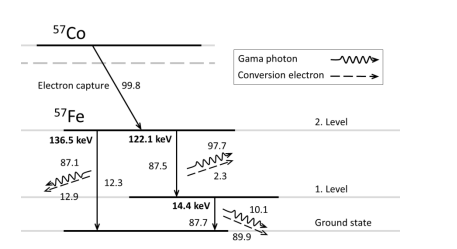
\includegraphics[scale=0.75, angle = 0]{./pictures/Fe57}
 \caption{Decay scheme of $^{57}$Co, taken from \cite{NOVAK2016thesis}.}
 \label{Fe57scheme}
 
\end{figure}

The MS spectrometer setup consists of several parts:
\begin{itemize}

\item Source of 14.4 keV gamma - $^{57}$Co radioactive nuclei built into a crystal lattice (usually in a rhodium matrix). The source is mounted on the transducer.
\item Transducer for Doppler modulation (figure \ref{transducer}). It usually consists of two coils surrounded by permanent magnets - one to drive the Doppler energy modulation and the other to measure the velocity \cite{mossInstr}. The system is driven by PID (proportional integral derivative) or MPC (model predictive control) controllers for precise velocity and energy control. The speed can be either constant or with constant acceleration.

\item Detector of transmitted/backscattered gamma radiation, conversion electrons or X-rays together with readout and evaluation electronics including amplifiers, single or multi-channel analysers, etc. It should also be noted that the conventional detectors mentioned above do not have sufficient energy resolution to distinguish the energy of perturbed states. For this reason, the count rates are synchronised with the Doppler energy modulation (actual modulated energy of the source), which is used to address the channels for spectrum accumulation. 


\end{itemize}
%The MS spectrometer setup consist of several parts:
%\begin{itemize}
%
%\item Source of 14.4 keV gamma - $^{57}$Co radioctive nuclei built-in crystal lattice (mostly in a rhodium matrice). The source is attached to the transducer.
%\item Transducer for doppler modulation (figure \ref{transducer}). It mostly consists of two coils surrounded by permanent magnets - one for driving the Doppler energy modulation and second for the velocity measurement \cite{mossInstr}. The system is driven by PID (proportional integral derivative) or MPC (model predictive control) controller for precise velocity and energy control. The velocity can be either constant or with constant acceleration.
%
%\item Detector of transmitted/backscattered gamma radiation, conversion electrons or X-ray along with readout and evaluation electronics including amplifiers, singlechannel or multichannel analysers etc. It is also necessary to consider, that the already mentioned conventional detectors have not sufficient energy resolution to distinguish the energy of perturbed states. Because of that, the count rates are synchronised with the Doppler energy modulation (actual modulated energy of the source), which is used to address the channels for spectra accumulation. 
%
%
%\end{itemize}

\begin{figure}[H]
 \centering
 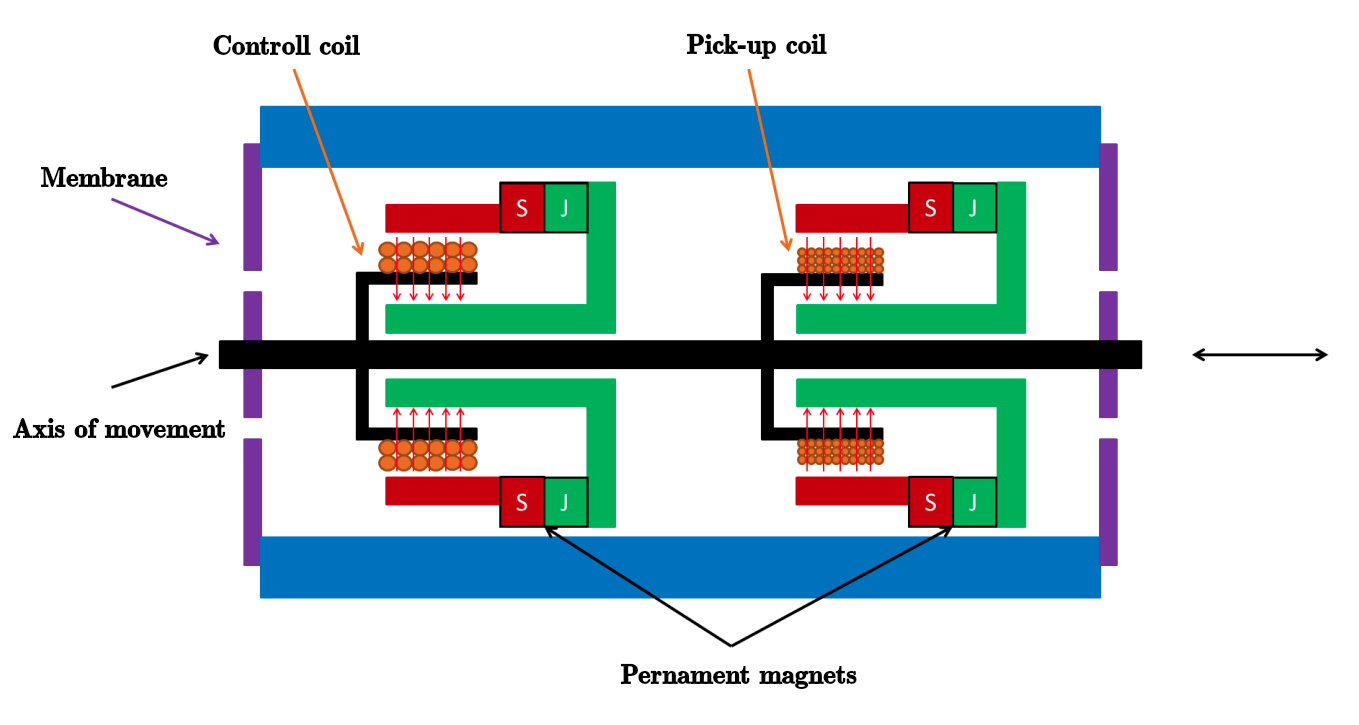
\includegraphics[scale=0.4, angle = 0]{./pictures/transducer}
 \caption{Transducer, taken from \cite{STEJSKAL2019thesis}.}
 \label{transducer}
 
\end{figure}


The diagram of the MS setup can be seen in the figure \ref{diagram}.

\begin{figure}[H]
 \centering
 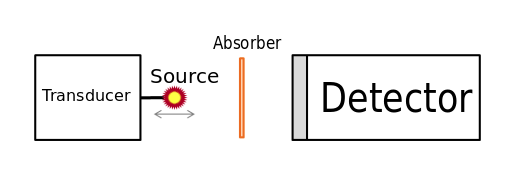
\includegraphics[scale=0.8, angle = 0]{./pictures/MSsetup.png}
 \caption{Diagram of the MS setup, taken and modified from \cite{NOVAK2016thesis}.}
 \label{diagram}
 
\end{figure}


\section{MS spectra effect and SNR}
The shape of the MS spectra can be modelled by Lorentzian curves. The singlet spectra in transmission geometry can be modelled by a single Lorentzian curve of the following form:

\begin{equation}
\begin{aligned}
L(v) = -I_{\textrm{MS}}\frac{(\frac{\Gamma}{2})^2}{(v - v_0)^2 + (\frac{\Gamma}{2})^2} + B
\end{aligned},
\label{lor}
\end{equation}
where $I_{\textrm{MS}}$ is the amplitude, the $\Gamma$ is the FWHM, and the $B$ is a background level. The Lorentzian in this form has the associated area $A$ equal to:

\begin{equation}
\begin{aligned}
A = \pi I_{\textrm{MS}} \Gamma
\end{aligned}
\label{area}
\end{equation}

There are two properties of MS spectra that characterise their quality: SNR and the effect $E_{\textrm{MS}}$. They can be calculated from the spectrum parameters using the following equations:

\begin{equation}
\begin{aligned}
\textrm{SNR}_{\textrm{MS}} = \frac{I_{\textrm{MS}}}{\sqrt{B}}
\end{aligned}
\label{SNR}
\end{equation}

\begin{equation}
\begin{aligned}
E_{\textrm{MS}} = \frac{I_{\textrm{MS}}}{B}
\end{aligned}
\label{effect}
\end{equation}



% %%%%%%%%%%%%%%%%%%%%%%%% End of file %%%%%%%%%%%%%%%%%%%%%%%%
